연결리스트는 배열이 아닌 다른 자료구조의 이해를 위한 기본적인 자료구조이다. 이 장에서는 연결리스트에 대한 학습과 더불어 자료구조를 공부할 때 어떠한 점을 생각해야 하는지 같이 살펴보겠다.

\section{자료구조를 왜 만드는가?}
자료구조는 `자료'와 `구조'가 합쳐진 말로, 자료와 구조가 모두 있어야 자료구조라 할 수 있다. 여기서 자료는 말 그대로 저장하고 싶은 데이터를 말하는 것이고, 구조는 어떤 `연산'을 얼마나 빠르게 처리할 수 있는지와 대응된다. 여기서 연산은 삽입, 삭제, 탐색과 같이 데이터와 상호작용하는 것이다.

배열은 가장 기본적인 자료구조로 볼 수 있다. 먼저, 배열은 저장하고자 하는 데이터 타입 \texttt{T}가 나열된 것이므로 당연히 `자료'가 있다.

\begin{figure}[h]
    \centering
    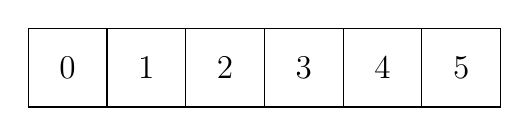
\begin{tikzpicture}
        \draw[step=1cm,black] (-3, 0) grid (3, 1);
        \node[font=\large] at (-2.5,0.5) {0};
        \node[font=\large] at (-1.5,0.5) {1};
        \node[font=\large] at (-0.5,0.5) {2};
        \node[font=\large] at (0.5,0.5) {3};
        \node[font=\large] at (1.5,0.5) {4};
        \node[font=\large] at (2.5,0.5) {5};
    \end{tikzpicture}
\end{figure}

`구조'에 해당하는 연산도 있을까? 사실, 처음 배열을 배웠을 때부터 연산을 하고 있었다. \texttt{cin >> arr[i]}를 반복문 안에서 반복하는 것은, 마지막 값이 $i-1$번 인덱스에 저장되어 있으므로, 자료구조의 끝에 삽입하는 연산과 같다. 실제로, 배열은 삽입, 삭제, 탐색 모두 가능하다.

모든 자료구조는 \textbf{특별한 장점}이 있어서 쓴다. 배열의 특별한 장점은 `임의 접근(random access)'을 빠르게 할 수 있다는 것이다. 정확히는, $O(1)$의 시간복잡도에 가능하다. 그리고, 모든 연산을 빠르게 처리할 수 있는 자료구조는 없다. 배열은 `임의 접근이 빠르다'는 장점을 얻은 대신에 `삽입과 삭제가 느리다'는 단점을 얻었다. 삽입과 삭제는 $O(N)$의 시간이 필요하다. 삽입을 위해서는 그보다 오른쪽에 있는 것들을 전부 오른쪽으로 한 칸 옮겨야 하고, 삭제를 위해서는 그보다 오른쪽에 있는 것들을 전부 왼쪽으로 한 칸 옯겨야 하기 때문이다. 연결리스트는 반대이다. `임의 접근이 느리다'는 단점이 있지만, `삽입과 삭제가 빠르다'는 장점을 얻었다.

\textbf{자료구조마다 장단점이 다르다는 것} 자체가 자료구조를 만들어야 하는 이유가 된다. 어떤 문제가 삽입과 삭제의 횟수가 매우 많고 랜덤 접근은 단 한 번도 하지 않는다면 연결리스트를 활용하는 것이 배열을 활용하는 것보다 더 나은 시간복잡도로 문제를 해결할 수 있을 것이다. 이 관점에서 보면 자료구조가 먼저 만들어진 것이 아니라, 문제가 먼저 제시되었고, 그 문제를 위한 자료구조가 개발된 것에 가깝다. 비유를 하자면, 자료구조는 수학에서 정리(Theorem)의 느낌이다. 정리를 쓰면 정리를 증명하는 과정을 건너뛸 수 있는 것처럼, 자료구조를 쓰면 문제에서 필요한 최적화를 건너뛸 수 있다.

정리하면, 문제를 보고 그 문제에서 `\textbf{여러 번 시행하기}를 요구하는 연산'을 빠르게 수행할 수 있는 자료구조를 사용하는 것이 `자료구조를 사용한 PS 문제의 해결'이라고 말할 수 있다. 따라서, 자료구조는 \underline{`빠르게 할 수 있는 연산'과 똑같은 개념}으로 받아들여야 한다. 

지금부터 우리가 배울 자료구조는 문제에서 `여러 번 시행하기'를 자주 요구해서 잘 알려진 것들이다. 특히, 이 파트의 자료구조는 특히 자주 요구하므로, 꼭 각 자료구조가 어떤 연산과 같은지 이해하고 다음으로 넘어가길 바란다.

\section{연결리스트}
연결리스트는 이름에서도 나타나듯이 연결을 통해 자료를 저장하는 방식이다. 

\begin{figure}[htbp]
    \centering
    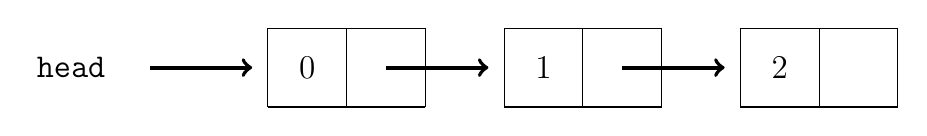
\begin{tikzpicture}
        \node[font=\large] at (-0.5,0.5) {\texttt{head}};
        \draw[step=1cm,black] (2, 0) grid (4, 1);
        \draw[step=1cm,black] (5, 0) grid (7, 1);
        \draw[step=1cm,black] (8, 0) grid (10, 1);
        \draw[->, line width=0.5mm] (0.5,0.5) -- (1.8,0.5);
        \node[font=\large] at (2.5,0.5) {0};
        \draw[->, line width=0.5mm] (3.5,0.5) -- (4.8,0.5);
        \node[font=\large] at (5.5,0.5) {1};
        \draw[->, line width=0.5mm] (6.5,0.5) -- (7.8,0.5);
        \node[font=\large] at (8.5,0.5) {2};
    \end{tikzpicture}
\end{figure}

하나의 데이터에는 데이터 뿐만 아니라 포인터가 붙어 있다. 이 하나의 쌍을 `노드(node)'라고 부를 것이다. 각 노드의 포인터는 다음 노드를 가리킴으로써 다음 노드와 `연결'하고, 특별히 헤드 포인터(그림에서 \texttt{head})가 시작 노드를 가리킨다. 이 헤드 포인터를 참조하면 연결리스트에 접근할 수 있는 것이다.

앞에서 연결리스트는 임의 접근을 포기하고 삽입과 삭제를 얻었다고 했다. 실제로 연결리스트에서 임의 접근, 삽입, 삭제가 어떻게 동작하는지 시뮬레이션해보자.

먼저 임의 접근이다. 임의로 $k$번째($0$-based) 위치에 접근하고 싶다면, 헤드 포인터가 가리키는 노드에서 $k$번 더 포인터를 통해 이동한 위치의 값을 가져오면 된다. 연결리스트에서는 발판들을 건너 넘어가는 것처럼, 순서대로 직접 가야 한다. 따라서 $k$번의 연산이 필요하고, 이를 점근 표기법으로 나타내면 $O(N)$이 되는 것이다.

두 번째로 삽입이다. \underline{`현재 노드 뒤'}(\Cref{pb: linked-list-insert})에 삽입하는 연산을 생각해보자. 그러면 새로 삽입되는 노드의 포인터를 현재 노드의 포인터로 바꾸고, 현재 노드의 포인터를 새로 삽입되는 노드로 바꾸면 된다. 아래 그림을 참고하자.

\begin{figure}[htbp]
    \centering
    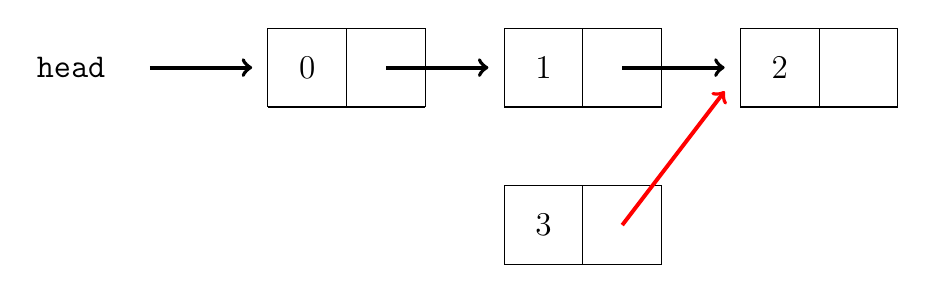
\begin{tikzpicture}
        \node[font=\large] at (-0.5,0.5) {\texttt{head}};
        \draw[step=1cm,black] (2, 0) grid (4, 1);
        \draw[step=1cm,black] (5, 0) grid (7, 1);
        \draw[step=1cm,black] (8, 0) grid (10, 1);
        \draw[->, line width=0.5mm] (0.5,0.5) -- (1.8,0.5);
        \node[font=\large] at (2.5,0.5) {0};
        \draw[->, line width=0.5mm] (3.5,0.5) -- (4.8,0.5);
        \node[font=\large] at (5.5,0.5) {1};
        \draw[->, line width=0.5mm] (6.5,0.5) -- (7.8,0.5);
        \node[font=\large] at (8.5,0.5) {2};
        
        \draw[step=1cm,black] (5, -2) grid (7, -1);
        \draw[->,red, line width=0.5mm] (6.5,-1.5) -- (7.8,0.2);
        \node[font=\large] at (5.5,-1.5) {3};
    \end{tikzpicture}

    \vspace{2em}

    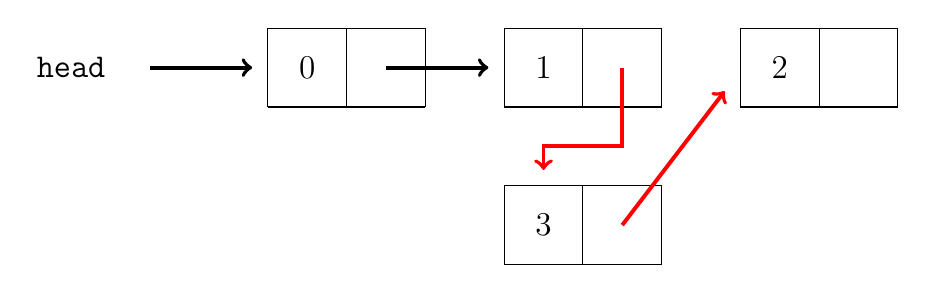
\begin{tikzpicture}
        \node[font=\large] at (-0.5,0.5) {\texttt{head}};
        \draw[step=1cm,black] (2, 0) grid (4, 1);
        \draw[step=1cm,black] (5, 0) grid (7, 1);
        \draw[step=1cm,black] (8, 0) grid (10, 1);
        \draw[->, line width=0.5mm] (0.5,0.5) -- (1.8,0.5);
        \node[font=\large] at (2.5,0.5) {0};
        \draw[->, line width=0.5mm] (3.5,0.5) -- (4.8,0.5);
        \node[font=\large] at (5.5,0.5) {1};
        \draw[->, red, line width=0.5mm] (6.5,0.5) -- (6.5, -0.5) -- (5.5, -0.5) -- (5.5,-0.8);
        \node[font=\large] at (8.5,0.5) {2};
        
        \draw[step=1cm,black] (5, -2) grid (7, -1);
        \draw[->,red, line width=0.5mm] (6.5,-1.5) -- (7.8,0.2);
        \node[font=\large] at (5.5,-1.5) {3};
    \end{tikzpicture}
\end{figure}

세 번째로 삭제이다. \underline{`현재 노드 뒤'}(\Cref{pb: linked-list-delete})에 있는 노드를 삭제하는 연산을 생각해보자. 그러면 현재 노드의 포인터를 현재 노드에서 바로 뒤에 있는 노드의 포인터로 바꾸고, 현재 노드 뒤에 있는 노드를 제거하면 된다. 아래 그림을 참고하자.

\begin{figure}[htbp]
    \centering
    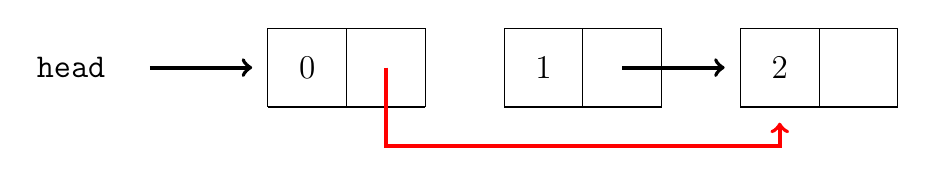
\begin{tikzpicture}
        \node[font=\large] at (-0.5,0.5) {\texttt{head}};
        \draw[step=1cm,black] (2, 0) grid (4, 1);
        \draw[step=1cm,black] (5, 0) grid (7, 1);
        \draw[step=1cm,black] (8, 0) grid (10, 1);
        \draw[->, line width=0.5mm] (0.5,0.5) -- (1.8,0.5);
        \node[font=\large] at (2.5,0.5) {0};
        \draw[->, red, line width=0.5mm] (3.5,0.5) -- (3.5, -0.5) -- (8.5, -0.5) -- (8.5,-0.2);
        \node[font=\large] at (5.5,0.5) {1};
        \draw[->, line width=0.5mm] (6.5,0.5) -- (7.8,0.5);
        \node[font=\large] at (8.5,0.5) {2};
    \end{tikzpicture}

    \vspace{2em}

    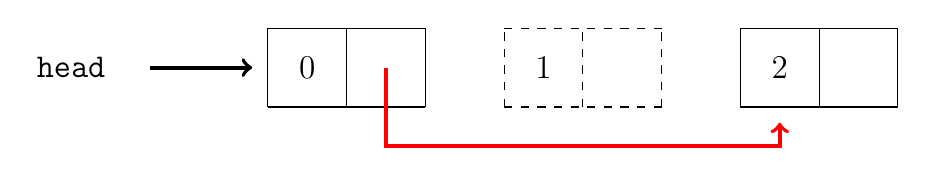
\begin{tikzpicture}
        \node[font=\large] at (-0.5,0.5) {\texttt{head}};
        \draw[step=1cm,black] (2, 0) grid (4, 1);
        \draw[step=1cm,dashed,black] (5, 0) grid (7, 1);
        \draw[step=1cm,black] (8, 0) grid (10, 1);
        \draw[->, line width=0.5mm] (0.5,0.5) -- (1.8,0.5);
        \node[font=\large] at (2.5,0.5) {0};
        \draw[->, red, line width=0.5mm] (3.5,0.5) -- (3.5, -0.5) -- (8.5, -0.5) -- (8.5,-0.2);
        \node[font=\large] at (5.5,0.5) {1};
        \node[font=\large] at (8.5,0.5) {2};
    \end{tikzpicture}
\end{figure}

\section{연결리스트의 구현}

연결리스트를 구현하려면 노드 구조체에 데이터 타입 \texttt{T}와 노드를 가리키는 포인터를 담아야 한다. 이렇게 되면 자기참조로써 컴파일러에서 무한루프에 빠지는거 아닐까? 하지만 포인터 자체는 unsigned long long int와 같고, 별(*) 연산자와 붙었을 때 구조체의 정보를 불러오기 때문에 이러한 일은 발생하지 않는다.

C는 클래스와 관련된 것이 하나도 존재하지 않아서 생성자와 소멸자를 사용할 수 없지만, C++에서는 구조체로 선언하였다 하더라도 구조체 자체가 클래스로 구현되어 있어서 생성자와 소멸자를 사용할 수 있다. 따라서 간단하게 \texttt{new}로 노드를 만들고, \texttt{del}로 노드를 제거할 수 있다. 메모리 누수 방지를 위해 노드 제거 작업은 꼭 필요하다.

이제 다음 코드 \Cref{code: linked-list}로 연결리스트의 구현을 보자. 포인터를 사용하는 자료구조의 구현은 본질적으로 이와 같고, 각 연산들의 로직만 다르므로 아래 구현 방식에는 익숙해쟀으면 한다. 실제 시험장에서 연결리스트를 구현할 일은 없겠지만, 포인터를 사용하는 자료구조 구현은 나중에 때때로 쓰이기 때문이다.

\begin{code} \label{code: linked-list}
연결리스트 구현 코드
\begin{lstlisting}
#include <bits/stdc++.h>
using namespace std;
int n;
    
struct Node {
    int a;
    Node *nxt;
    Node() {
        a = 0;
        nxt = NULL;
    }
};
Node *head = new Node();
    
void add(Node *node, int val) {
    Node *added = new Node();
    added->a = val;
    added->nxt = node->nxt;
    node->nxt = added;
}
    
void rem(Node *node) {
    Node *tar = node->nxt;
    if (tar == NULL) return;
    node->nxt = tar->nxt;
    delete tar;
}
\end{lstlisting}
\end{code}

구조체 \texttt{Node} 안에 선언된 \texttt{Node()} 함수는 생성자로, \texttt{new}를 사용하여 구조체 변수를 만들 때 자동으로 실행된다. 함수 이름을 구조체 이름과 똑같이 설정하면 된다. 만약, 소멸자가 필요하다면 \texttt{~Node()}와 같이 물결을 붙여서 함수 이름을 정하면 된다. 이 소멸자는 \texttt{delete}를 사용하여 구조체 변수를 제거할 때 자동으로 실행된다.

\section{STL의 연결리스트}
STL에는 연결리스트가 있다. \url{https://en.cppreference.com/w/cpp/container/list}에 가면 어떤 함수를 지원하고 어떻게 사용하는지, 시간복잡도까지 모두 확인할 수 있다. 그 중에서 중요한 함수만을 소개하겠다. 그 전에 몇 가지 용어를 정의하자. STL container에서는 C언어의 포인터와 같은 기능을 하는 것을 \textbf{iterator}라고 표현한다. 그리고 iterator로 표현된 구간은 기본적으로 반열린구간 $[s, e)$로 처리된다. 또, 저장하는 데이터의 자료형은 \texttt{T}로 표기한다. 즉, 함수 인자에 \texttt{T}가 있다면 데이터를 함수 인자로 넣으라는 뜻이다.

\begin{itemize}
    \item \texttt{front()}를 통해 제일 앞의 노드를 참조할 수 있다.
    \item \texttt{back()}를 통해 제일 뒤의 노드를 참조할 수 있다.
    \item \texttt{begin()}를 통해 제일 앞의 노드를 가리키는 포인터를 참조할 수 있다.
    \item \texttt{end()}를 통해 제일 뒤의 노드의 \textbf{다음 노드}를 가리키는 포인터를 참조할 수 있다.
    \item \texttt{push\_front(T)}를 통해 제일 앞에 새로운 데이터를 추가할 수 있다.
    \item \texttt{push\_back(T)}를 통해 제일 뒤에 새로운 데이터를 추가할 수 있다.
    \item \texttt{pop\_front()}를 통해 제일 앞의 노드를 제거할 수 있다.
    \item \texttt{pop\_back()}를 통해 제일 뒤의 노드를 제거할 수 있다.
    \item \texttt{erase(iterator)}를 통해 포인터(iterator)가 가리키는 노드를 제거할 수 있다.
    \item \texttt{insert(iterator, T)}를 통해 포인터(iterator)의 위치에 새로운 데이터를 추가할 수 있다.
    \item \texttt{empty()}를 통해 비어있는지 여부를 확인할 수 있다.
    \item \texttt{size()}를 통해 저장된 데이터의 개수를 확인할 수 있다.
    \item \texttt{clear()}를 통해 모든 데이터를 지울 수 있다.
\end{itemize}

상술된 함수들은 대부분의 STL container에서 공통적으로 존재하는 함수들이다. 따라서 같은 이름의 함수를 앞으로 계속 만나게 된다. 그리고, 각 함수들이 매번 비슷한 기능을 하므로 다양한 STL container를 만나면서 점차 친숙해지면 된다.

코드에서 사용하는 방법은 다음 예시 \Cref{code: stl-list-ex}를 참고하라.

\begin{code} \label{code: stl-list-ex}
\texttt{std::list}의 예시 코드
\begin{lstlisting}
#include <algorithm>
#include <iostream>
#include <list>
    
int main()
{
    // Create a list containing integers
    std::list<int> l = {7, 5, 16, 8};
    
    // Add an integer to the front of the list
    l.push_front(25);
    // Add an integer to the back of the list
    l.push_back(13);
    
    // Insert an integer before 16 by searching
    auto it = std::find(l.begin(), l.end(), 16);
    if (it != l.end())
        l.insert(it, 42);
    
    // Print out the list
    std::cout << "l = { ";
    for (int n : l)
        std::cout << n << ", ";
    std::cout << "};\n";
}
\end{lstlisting}
\end{code}

\section{연습문제 A}
\begin{problem} \label{pb: linked-list-insert}
    연결리스트에서 헤드 포인터와 삽입하고 싶은 위치의 인덱스 $k$($0$-based)가 주어질 때 연산의 시간복잡도는 무엇인가? 삽입이 아닌 삭제에서는 어떠한가?
\end{problem}
\begin{problem} \label{pb: linked-list-delete}
    연결리스트에서 \textbf{현재 포인터}를 $O(1)$에 삭제하려면 어떻게 수정하면 될까? 방법을 고안하고 직접 구현해보라.
\end{problem}

\section{연습문제 B}
\begin{problem}
    (5680번) \url{https://www.acmicpc.net/problem/5680}
\end{problem}
\begin{problem}
    (3294번) \url{https://www.acmicpc.net/problem/3294}
\end{problem}
\begin{problem}
    (4621번) \url{https://www.acmicpc.net/problem/4621}
\end{problem}
\begin{problem}
    (6542번) \url{https://www.acmicpc.net/problem/6542}
\end{problem}
\begin{problem}
    (22645번) \url{https://www.acmicpc.net/problem/22645}
\end{problem}
\begin{problem}
    (23309번) \url{https://www.acmicpc.net/problem/23309}
\end{problem}
\begin{problem}
    (25252번) \url{https://www.acmicpc.net/problem/25252}
\end{problem}
\begin{problem}
    (30885번) \url{https://www.acmicpc.net/problem/30885}
\end{problem}
\begin{problem}
    (31857번) \url{https://www.acmicpc.net/problem/31857}
\end{problem}
\begin{problem}
    (3217번) \url{https://www.acmicpc.net/problem/3217}
\end{problem}

\begin{problem}
    (21201번*) \url{https://www.acmicpc.net/problem/21201}
\end{problem}
\begin{problem}
    (17820번*) \url{https://www.acmicpc.net/problem/17820}
\end{problem}
\begin{problem}
    (23774번*) \url{https://www.acmicpc.net/problem/23774}
\end{problem}
\begin{problem}
    (28974번*) \url{https://www.acmicpc.net/problem/28974}
\end{problem}

\section{연습문제 C}
\begin{problem}
    (26032번) \url{https://www.acmicpc.net/problem/26032}
\end{problem}
\begin{problem}
    (24971번*) \url{https://www.acmicpc.net/problem/24971}
\end{problem}
\begin{problem}
    (17692번**) \url{https://www.acmicpc.net/problem/17692}
\end{problem}